% !TEX root = ../main.tex
% File: chapters_part1/chap3_3.tex
% Nội dung cho Phần 3.3: Mạng Nơ-ron Hồi tiếp (RNNs, LSTMs, GRUs)

\section{Mạng Nơ-ron Hồi tiếp (RNNs, LSTMs, GRUs)}
\label{sec:rnns}

Nếu một mạng nơ-ron truyền thẳng (Feed-Forward Neural Network - FNN) là bộ não xử lý thông tin một cách tức thời, thì Mạng Nơ-ron Hồi tiếp (Recurrent Neural Network - RNN) là bộ não có \textbf{trí nhớ}. Đây là ý tưởng đột phá cho phép mạng nơ-ron xử lý các chuỗi có độ dài thay đổi, một đặc tính cố hữu của ngôn ngữ.

\subsection{Mạng Nơ-ron Hồi tiếp Đơn giản (Vanilla RNN)}
\label{ssec:vanilla_rnn}

\subsubsection{Tư duy cốt lõi: Vòng lặp của Trí nhớ}
Một mạng FNN thông thường xử lý mỗi đầu vào một cách độc lập. Nó không có khái niệm về "thời gian" hay "thứ tự". Để hiểu một câu, chúng ta cần xử lý các từ theo đúng thứ tự và ghi nhớ những gì đã đọc.

RNN thực hiện điều này bằng một cơ chế đơn giản nhưng thanh lịch: một \textbf{vòng lặp (loop)}. Tại mỗi bước thời gian $t$, mạng không chỉ nhận đầu vào hiện tại $x_t$ (vector của từ thứ $t$), mà còn nhận cả \textbf{đầu ra của chính nó từ bước thời gian trước đó}, $h_{t-1}$. Đầu ra này, gọi là \textbf{trạng thái ẩn (hidden state)}, đóng vai trò như một "bộ nhớ" tóm tắt lại toàn bộ thông tin đã được xử lý cho đến thời điểm đó.

\begin{center}
    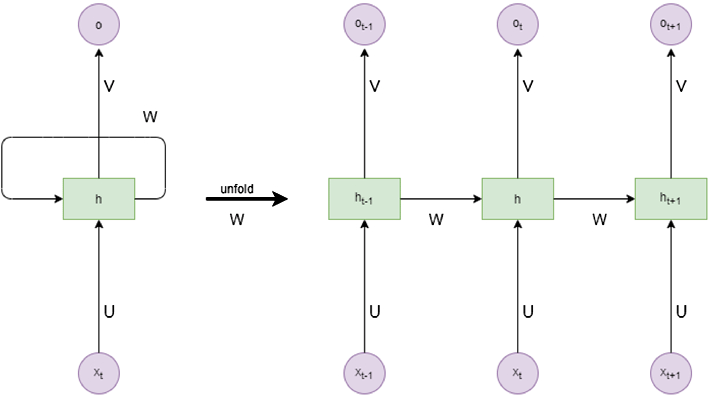
\includegraphics[width=0.9\textwidth]{rnn_unrolled.png}
    \captionof{figure}{Kiến trúc của một RNN. Bên trái là dạng nén với vòng lặp. Bên phải là dạng "trải ra theo thời gian" (unrolled), cho thấy cách trạng thái ẩn $h$ được truyền từ bước này sang bước tiếp theo.}
    \label{fig:rnn_unrolled}
\end{center}

\subsubsection{Kiến trúc và Dòng chảy Dữ liệu}
Tại mỗi bước thời gian $t$:
\begin{enumerate}
    \item \textbf{Đầu vào:} Vector từ $x_t$ và trạng thái ẩn từ bước trước $h_{t-1}$.
    \item \textbf{Tính toán trạng thái ẩn mới:} Trạng thái ẩn mới, $h_t$, được tính bằng cách kết hợp $x_t$ và $h_{t-1}$ qua một phép biến đổi tuyến tính và một hàm kích hoạt (thường là `tanh`).
        \begin{equation}
            h_t = \tanh(W_{hh} h_{t-1} + W_{xh} x_t + b_h)
        \end{equation}
        Trong đó, $W_{hh}$ và $W_{xh}$ là các ma trận trọng số được \textbf{chia sẻ (shared)} trên tất cả các bước thời gian. Đây là điểm mấu chốt: mô hình học một bộ quy tắc duy nhất để cập nhật trí nhớ, bất kể vị trí trong chuỗi.
    \item \textbf{Tạo đầu ra (tùy chọn):} Một đầu ra $y_t$ có thể được tạo ra từ trạng thái ẩn $h_t$.
        \begin{equation}
            y_t = W_{hy} h_t + b_y
        \end{equation}
\end{enumerate}
\begin{tcolorbox}[
    title=Ghi chú sâu về Thiết kế của RNN Đơn giản,
    colback=green!5!white, colframe=green!50!black, fonttitle=\bfseries
]
\textbf{1. Tại sao phải Chia sẻ Trọng số?} \\
Đây là nguyên lý nền tảng của RNN. Việc sử dụng cùng một bộ trọng số ($W_{hh}, W_{xh}$) ở mọi bước thời gian cho phép mô hình học một quy tắc cập nhật \textbf{tổng quát} có thể áp dụng cho bất kỳ vị trí nào trong chuỗi. Nếu mỗi bước thời gian có một bộ trọng số riêng, mô hình sẽ:
\begin{itemize}
    \item Có số lượng tham số khổng lồ, phụ thuộc vào độ dài chuỗi, khiến việc huấn luyện bất khả thi.
    \item Không thể tổng quát hóa cho các chuỗi có độ dài khác với dữ liệu huấn luyện. Nó sẽ chỉ học thuộc lòng các mẫu ở các vị trí cố định.
\end{itemize}
Việc chia sẻ trọng số chính là cách RNN học được một "thuật toán" xử lý chuỗi.

\textbf{2. Tại sao dùng hàm `tanh`?} \\
Hàm `tanh` đưa đầu ra về khoảng $[-1, 1]$. Điều này giúp giữ cho các giá trị trong trạng thái ẩn không bị tăng hoặc giảm quá nhanh, tức là kiểm soát dòng chảy thông tin một cách tương đối ổn định. Nếu dùng `ReLU` (vốn không có giới hạn trên), trạng thái ẩn có thể tăng lên vô hạn, làm cho vấn đề bùng nổ gradient trở nên trầm trọng hơn rất nhiều. `tanh` hoạt động như một cơ chế "bão hòa" tự nhiên.
\end{tcolorbox}

\subsubsection{Huấn luyện RNN: Lan truyền ngược theo thời gian (BPTT)}
\label{sssec:bptt}
Quá trình huấn luyện một RNN cũng dựa trên việc tối thiểu hóa một hàm mất mát, nhưng có một sự phức tạp hơn so với mạng FNN.
\begin{itemize}
    \item \textbf{Hàm Mất mát:} Tại mỗi bước thời gian $t$, mô hình tạo ra một dự đoán $y_t$. Lỗi tại bước đó, $\mathcal{L}_t$, được tính toán bằng cách so sánh $y_t$ với nhãn thật tương ứng. \textbf{Tổng lỗi} cho toàn bộ chuỗi là tổng của các lỗi tại mỗi bước: $\mathcal{L} = \sum_{t=1}^{T} \mathcal{L}_t$.
    
    \item \textbf{Lan truyền ngược theo thời gian (Backpropagation Through Time - BPTT):} Để tính toán gradient của tổng lỗi $\mathcal{L}$ theo các trọng số (ví dụ $W_{hh}$), chúng ta phải sử dụng một biến thể của backpropagation gọi là BPTT. Gradient tại một bước thời gian $t$ không chỉ phụ thuộc vào lỗi tại bước $t$, mà còn phụ thuộc vào gradient từ tất cả các bước thời gian \textit{trong tương lai} ($t+1, t+2, \dots, T$) được truyền ngược lại thông qua trạng thái ẩn $h$.
    
    \item \textbf{Vấn đề của BPTT:} Chính việc gradient phải được truyền ngược qua nhiều bước thời gian này là nguyên nhân gây ra các vấn đề nan giải được thảo luận dưới đây.
\end{itemize}

\subsubsection{Vấn đề nan giải: Vanishing và Exploding Gradients}
RNN về lý thuyết có thể học các phụ thuộc tầm xa. Tuy nhiên, trong thực tế, chúng gặp rất nhiều khó khăn. Quá trình huấn luyện RNN sử dụng thuật toán lan truyền ngược theo thời gian (Backpropagation Through Time - BPTT). Khi lan truyền gradient lỗi ngược qua nhiều bước thời gian, gradient này phải đi qua phép nhân lặp đi lặp lại với ma trận trọng số $W_{hh}$.

\begin{itemize}
    \item \textbf{Vanishing Gradients (Triệt tiêu Gradient):} Nếu các giá trị trong $W_{hh}$ nhỏ (norm < 1), sau nhiều lần nhân, gradient sẽ co lại và tiến dần về 0.
        \begin{itemize}
            \item \textbf{Hậu quả:} Mạng không thể học được các phụ thuộc giữa các từ ở xa nhau. Tín hiệu lỗi từ tương lai không thể lan truyền đủ xa về quá khứ để cập nhật trọng số một cách có ý nghĩa. RNN trở nên "thiển cận", chỉ nhớ được vài bước gần nhất. Đây là vấn đề nghiêm trọng nhất.
        \end{itemize}
    \item \textbf{Exploding Gradients (Bùng nổ Gradient):} Nếu các giá trị trong $W_{hh}$ lớn (norm > 1), gradient sẽ tăng theo cấp số nhân và trở nên khổng lồ.
        \begin{itemize}
            \item \textbf{Hậu quả:} Gây ra các bước cập nhật trọng số cực lớn, làm cho quá trình huấn luyện trở nên mất ổn định. Vấn đề này có thể được giải quyết phần nào bằng kỹ thuật \textit{gradient clipping} (cắt bớt gradient nếu nó vượt quá một ngưỡng).
        \end{itemize}
\end{itemize}

Vấn đề triệt tiêu gradient đã thúc đẩy sự ra đời của các kiến trúc RNN phức tạp hơn, có khả năng kiểm soát dòng chảy thông tin một cách thông minh hơn.

\subsection{Long Short-Term Memory (LSTM)}
\label{ssec:lstm}
LSTM, được giới thiệu bởi Hochreiter \& Schmidhuber vào năm 1997 \cite{hochreiter1997long}, là một biến thể đặc biệt của RNN, được thiết kế một cách xuất sắc để giải quyết vấn đề triệt tiêu gradient. Nó đã trở thành kiến trúc thống trị cho các bài toán chuỗi trong gần hai thập kỷ.

\subsubsection{Tư duy cốt lõi: Các Cổng và Trạng thái Ô nhớ}
Ý tưởng thiên tài của LSTM là giới thiệu một "làn đường cao tốc" cho thông tin, gọi là \textbf{trạng thái ô nhớ (cell state)}, ký hiệu là $C_t$. Trạng thái ô nhớ này chạy dọc theo toàn bộ chuỗi, chỉ với một vài tương tác tuyến tính nhỏ. Thông tin có thể dễ dàng chảy trên làn đường này mà không bị thay đổi nhiều.

LSTM có khả năng thêm hoặc bớt thông tin ra khỏi trạng thái ô nhớ một cách cẩn thận, được điều khiển bởi các cấu trúc gọi là \textbf{cổng (gates)}. Cổng là một cách để thông tin có thể đi qua một cách tùy chọn. Chúng bao gồm một lớp mạng sigmoid và một phép nhân theo từng phần tử (element-wise multiplication).

\begin{center}
    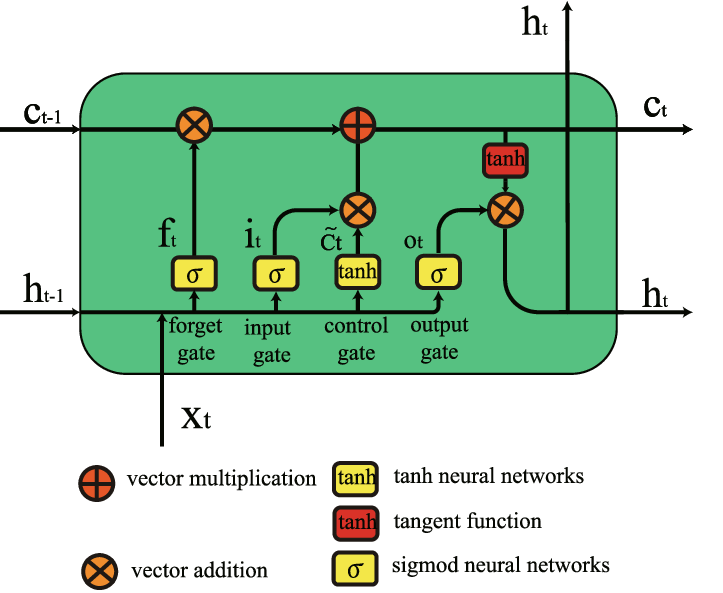
\includegraphics[width=0.7\textwidth]{lstm_cell_diagram.png}
    \captionof{figure}{Sơ đồ chi tiết của một ô nhớ LSTM. Nó bao gồm 3 cổng chính (Quên, Nạp, Xuất) và một trạng thái ô nhớ $C_t$ chạy ngang.}
    \label{fig:lstm_cell_diagram}
\end{center}

Một ô LSTM có ba cổng để bảo vệ và kiểm soát trạng thái ô nhớ:

\paragraph{1. Cổng Quên (Forget Gate - $f_t$)}
Cổng này quyết định xem thông tin nào nên được \textbf{loại bỏ} khỏi trạng thái ô nhớ của bước trước.
$$ f_t = \sigma(W_f [h_{t-1}, x_t] + b_f) $$
Nó nhìn vào $h_{t-1}$ và $x_t$, và xuất ra một vector số từ 0 đến 1 cho mỗi số trong trạng thái ô nhớ $C_{t-1}$. Số 1 có nghĩa là "giữ lại hoàn toàn", số 0 có nghĩa là "quên hoàn toàn".

\paragraph{2. Cổng Nạp (Input Gate - $i_t$)}
Cổng này quyết định xem thông tin mới nào nên được \textbf{lưu trữ} vào trạng thái ô nhớ. Quá trình này có hai bước:
\begin{enumerate}
    \item Một lớp sigmoid (cổng nạp) quyết định những giá trị nào chúng ta sẽ cập nhật.
        $$ i_t = \sigma(W_i [h_{t-1}, x_t] + b_i) $$
    \item Một lớp `tanh` tạo ra một vector các giá trị ứng viên mới, $\tilde{C}_t$, có thể được thêm vào trạng thái.
        $$ \tilde{C}_t = \tanh(W_C [h_{t-1}, x_t] + b_C) $$
\end{enumerate}

\paragraph{3. Cập nhật Trạng thái Ô nhớ}
Bây giờ, chúng ta cập nhật trạng thái ô nhớ cũ $C_{t-1}$ thành trạng thái mới $C_t$.
$$ C_t = f_t \odot C_{t-1} + i_t \odot \tilde{C}_t $$
Ký hiệu $\odot$ là phép nhân theo từng phần tử. Chúng ta nhân trạng thái cũ với $f_t$ (quên đi những gì đã quyết định quên), sau đó cộng với $i_t \odot \tilde{C}_t$ (thêm vào những thông tin mới đã quyết định nạp). Phép cộng này chính là chìa khóa giúp gradient có thể chảy ngược một cách dễ dàng, giải quyết vấn đề triệt tiêu gradient.

\paragraph{4. Cổng Xuất (Output Gate - $o_t$)}
Cuối cùng, cổng này quyết định xem chúng ta sẽ xuất ra cái gì. Đầu ra này sẽ dựa trên trạng thái ô nhớ của chúng ta, nhưng sẽ là một phiên bản đã được "lọc".
\begin{enumerate}
    \item Một lớp sigmoid quyết định phần nào của trạng thái ô nhớ chúng ta sẽ xuất ra.
        $$ o_t = \sigma(W_o [h_{t-1}, x_t] + b_o) $$
    \item Chúng ta đưa trạng thái ô nhớ qua hàm `tanh` (để đưa giá trị về khoảng [-1, 1]) và nhân nó với đầu ra của cổng sigmoid, để chỉ xuất ra những phần chúng ta muốn.
        $$ h_t = o_t \odot \tanh(C_t) $$
\end{enumerate}
Trạng thái ẩn mới $h_t$ này sẽ được sử dụng để dự đoán đầu ra $y_t$ và được truyền tới bước thời gian tiếp theo.
\paragraph{Phân tích: Tại sao LSTM hoạt động?}
Sự kỳ diệu của LSTM nằm ở cách nó tách biệt dòng chảy thông tin và kiểm soát nó một cách tinh vi:
\begin{itemize}
    \item \textbf{Con đường cao tốc Gradient (Gradient Highway):} Nhìn lại công thức cập nhật trạng thái ô nhớ: $C_t = f_t \odot C_{t-1} + i_t \odot \tilde{C}_t$. Thành phần quan trọng nhất là phép cộng. Trong quá trình lan truyền ngược, gradient của $C_t$ đối với $C_{t-1}$ có một thành phần trực tiếp là $f_t$. Do $f_t$ được điều khiển bởi hàm sigmoid, giá trị của nó thường không bị quá nhỏ hoặc quá lớn. Điều này tạo ra một "con đường" gần như không bị cản trở để gradient có thể chảy ngược qua nhiều bước thời gian mà không bị triệt tiêu hoàn toàn. RNN đơn giản chỉ có phép nhân lặp đi lặp lại, khiến gradient dễ dàng biến mất.
    
    \item \textbf{Phân vai Trí nhớ:} LSTM tạo ra một sự phân vai rõ ràng:
        \begin{itemize}
            \item \textbf{Trạng thái Ô nhớ ($C_t$):} Đóng vai trò như \textbf{trí nhớ dài hạn}. Nó chứa tất cả thông tin tích lũy được. Nó có thể được thay đổi một cách cẩn trọng thông qua các cổng, nhưng bản chất là một "kho lưu trữ".
            \item \textbf{Trạng thái Ẩn ($h_t$):} Đóng vai trò như \textbf{trí nhớ làm việc (working memory)}. Nó là một phiên bản "đã lọc" của trí nhớ dài hạn, chỉ chứa những thông tin liên quan đến quyết định cần đưa ra \textit{tại thời điểm hiện tại}. Việc tách biệt này cho phép mô hình vừa lưu trữ thông tin từ rất xa trong quá khứ ($C_t$), vừa tập trung vào những gì cần thiết cho bước tiếp theo ($h_t$).
        \end{itemize}
\end{itemize}
\subsection{Gated Recurrent Unit (GRU)}
\label{ssec:gru}
Được giới thiệu bởi Cho và các cộng sự vào năm 2014, GRU \cite{cho2014learning} là một biến thể của LSTM với kiến trúc đơn giản hơn. Nó kết hợp cổng quên và cổng nạp thành một "cổng cập nhật" duy nhất, và cũng hợp nhất trạng thái ô nhớ và trạng thái ẩn.

\paragraph{Tư duy cốt lõi}
GRU giữ lại tinh thần của LSTM là sử dụng các cổng để điều khiển dòng chảy thông tin, nhưng với ít tham số hơn, giúp việc huấn luyện nhanh hơn và hiệu quả hơn trên các bộ dữ liệu nhỏ.

GRU có hai cổng chính:
\paragraph{1. Cổng Cập nhật (Update Gate - $z_t$)}
Cổng này có vai trò tương tự cả cổng quên và cổng nạp trong LSTM. Nó quyết định xem bao nhiêu thông tin từ trạng thái ẩn quá khứ ($h_{t-1}$) nên được giữ lại, và bao nhiêu thông tin mới ($\tilde{h}_t$) nên được thêm vào.
$$ z_t = \sigma(W_z [h_{t-1}, x_t] + b_z) $$

\paragraph{2. Cổng Reset (Reset Gate - $r_t$)}
Cổng này quyết định xem bao nhiêu phần của trạng thái ẩn quá khứ nên được "quên" đi khi tính toán trạng thái ứng viên mới.
$$ r_t = \sigma(W_r [h_{t-1}, x_t] + b_r) $$

\paragraph{Tính toán Trạng thái}
\begin{enumerate}
    \item Trạng thái ẩn ứng viên mới $\tilde{h}_t$ được tính toán, nhưng có sử dụng cổng reset để kiểm soát ảnh hưởng của $h_{t-1}$.
        $$ \tilde{h}_t = \tanh(W_h [r_t \odot h_{t-1}, x_t] + b_h) $$
        Nếu cổng reset $r_t$ gần bằng 0, mô hình sẽ gần như bỏ qua hoàn toàn thông tin quá khứ và chỉ tập trung vào đầu vào hiện tại $x_t$ để tạo trạng thái mới.
    \item Trạng thái ẩn cuối cùng $h_t$ là một sự nội suy tuyến tính giữa trạng thái cũ $h_{t-1}$ và trạng thái ứng viên mới $\tilde{h}_t$, được điều khiển bởi cổng cập nhật $z_t$.
        $$ h_t = (1 - z_t) \odot h_{t-1} + z_t \odot \tilde{h}_t $$
\end{enumerate}
\paragraph{Phân tích: Sự đánh đổi của GRU}
GRU là một ví dụ tuyệt vời về việc đơn giản hóa kiến trúc mà vẫn giữ được hiệu quả cốt lõi.
\begin{itemize}
    \item \textbf{Cổng Reset - Cơ chế "Khởi động lại Ngữ cảnh":} Cổng reset ($r_t$) cho phép GRU bỏ qua hoàn toàn trí nhớ quá khứ khi cần thiết. Hãy tưởng tượng khi đọc một đoạn văn và gặp một dấu chấm hết câu, bắt đầu một câu mới với chủ đề khác. Cổng reset có thể học cách "kích hoạt" (đưa giá trị về gần 0) tại những điểm chuyển tiếp này, cho phép trạng thái ứng viên mới $\tilde{h}_t$ được hình thành chủ yếu từ đầu vào hiện tại $x_t$, tạo ra một khởi đầu mới cho ngữ cảnh.
    
    \item \textbf{Cổng Cập nhật - Nội suy mượt mà:} Công thức $h_t = (1 - z_t) \odot h_{t-1} + z_t \odot \tilde{h}_t$ hoạt động như một bộ điều khiển "rò rỉ". Khi $z_t$ gần bằng 0, phần lớn $h_{t-1}$ sẽ được sao chép trực tiếp sang $h_t$, giúp thông tin được bảo tồn qua các bước thời gian dài. Ngược lại, khi $z_t$ gần bằng 1, thông tin mới sẽ được ưu tiên. Sự cân bằng này giúp GRU mô hình hóa các phụ thuộc dài hạn một cách hiệu quả, dù không có một "trạng thái ô nhớ" riêng biệt.
\end{itemize}
Việc gộp trạng thái ô nhớ và trạng thái ẩn làm cho GRU mất đi một chút sức mạnh biểu diễn so với LSTM, nhưng chính sự đơn giản này lại giúp nó huấn luyện nhanh hơn và đôi khi tổng quát hóa tốt hơn trên các tập dữ liệu nhỏ.
\begin{tcolorbox}[
    title=So sánh LSTM và GRU,
    colback=green!5!white, colframe=green!60!black, fonttitle=\bfseries
]
\begin{tabular}{p{0.45\linewidth} | p{0.45\linewidth}}
    \textbf{LSTM} & \textbf{GRU} \\
    \hline
    Có 3 cổng: Quên, Nạp, Xuất. & Có 2 cổng: Cập nhật, Reset. \\
    \hline
    Có trạng thái ô nhớ ($C_t$) và trạng thái ẩn ($h_t$) riêng biệt. & Chỉ có một trạng thái ẩn ($h_t$). \\
    \hline
    Nhiều tham số hơn. & Ít tham số hơn. \\
    \hline
    Linh hoạt và mạnh mẽ hơn về mặt lý thuyết. & Nhanh hơn, hiệu quả hơn về mặt tính toán và cần ít dữ liệu hơn để tổng quát hóa. \\
    \hline
    \textbf{Khi nào dùng?} Không có quy tắc tuyệt đối. GRU là một lựa chọn khởi đầu tốt. Nếu bài toán rất phức tạp và có đủ dữ liệu, LSTM có thể cho hiệu năng nhỉnh hơn.
\end{tabular}
\end{tcolorbox}